% DOCUMENT TYPE: PRESENTATION
\documentclass[12pt,aspectratio=169]{beamer}

% PACKAGES TO USE
\usepackage[utf8]{inputenc}
\usepackage[spanish]{babel}
\usepackage{lastpage}
\usepackage{subcaption}
\usepackage[export]{adjustbox}

% CONFIGURATIONS
\setbeamertemplate{footline}[frame number]

% PRESENTATION INFO
\title[Red Neuronal Convolucional Adversarial]{Reconstrucción de Huellas Dactilares Digitales Utilizando un Modelo Generativo Adversarial Convolucional}
\author[Andrade, C]{Cristian Yesid Andrade Hernández}
\institute[Universidad de los Andes]
{ 
\includegraphics[width=5cm]{figs/uniandes_logo.png} }

\date{\today}

% DOCUMENT
\begin{document}

% ==== INIT SLIDE ====
\frame[plain]{\titlepage}


% ==== SLIDE 3 ====
\begin{frame}{Introducción}

    La captura digital de huellas dactilares puede resultar en imágenes deterioradas.
    \vspace{3mm}

    \begin{figure}[h]
        \begin{subfigure}{0.3\textwidth}
            \centering
            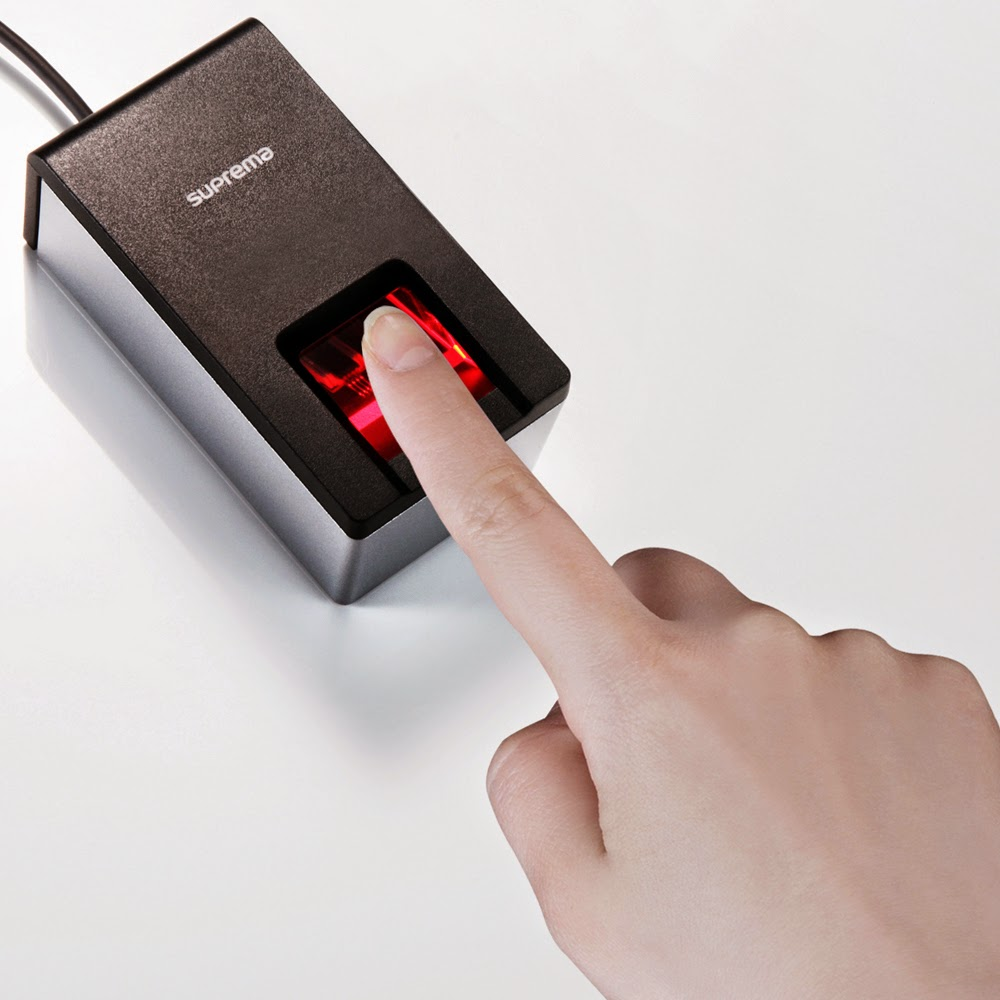
\includegraphics[scale=0.12]{figs/dedo_lector_biometrico.jpg}
        \end{subfigure}
        \begin{subfigure}{0.14\textwidth}
            \centering
            $\longrightarrow$
        \end{subfigure}
        \begin{subfigure}{0.23\textwidth}
            \centering
            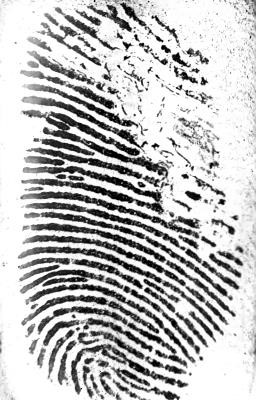
\includegraphics[scale=0.32]{figs/deteriorada_1.jpg}
            \caption{Huella Incompleta}
        \end{subfigure}
        \begin{subfigure}{0.23\textwidth}
            \centering
            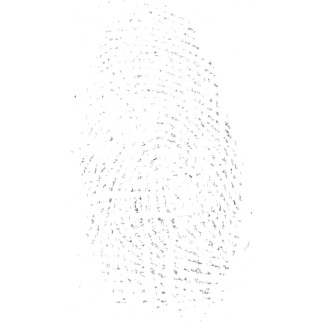
\includegraphics[scale=0.3]{figs/deteriorada_0.png}
            \caption{Huella Borrosa}
        \end{subfigure}
    \end{figure}

\end{frame}

% ==== SLIDE 4 ====
\begin{frame}{Introducción}

    Se propone reconstruir y mejorar la huella digital obtenida mediante red neuronal convolucional.
    \vspace{3mm}

    \begin{figure}[h]
        \begin{subfigure}{0.58\textwidth}
            \centering
            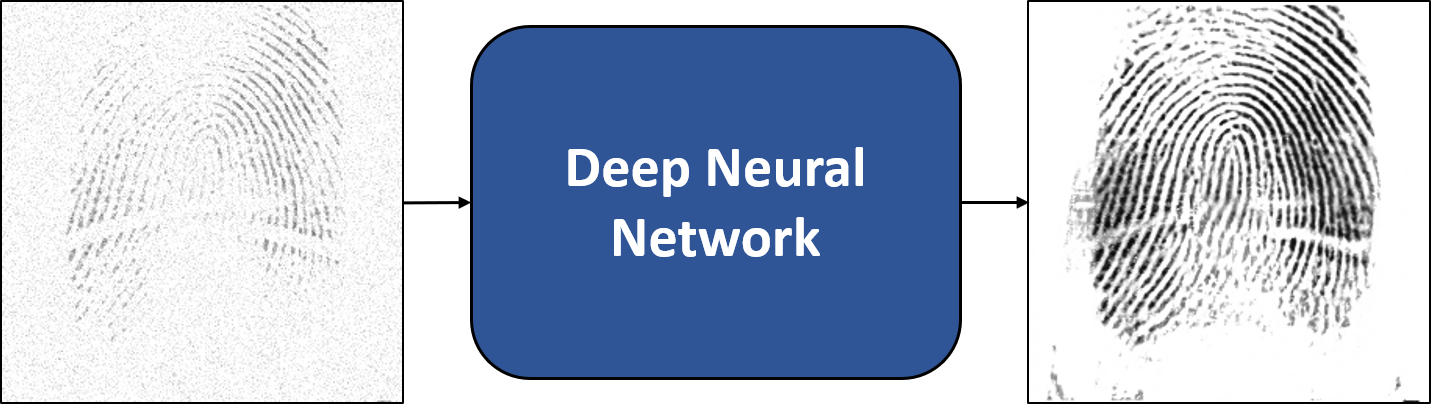
\includegraphics[scale=0.34]{figs/end_to_end.png}  
            \caption{Modelo end to end}
        \end{subfigure}
        \begin{subfigure}{0.38\textwidth}
            \centering
            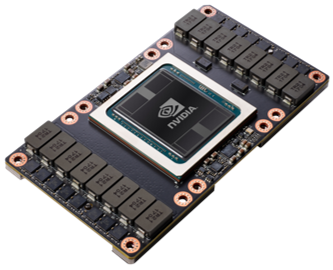
\includegraphics[scale=0.28]{figs/nvidia_card.png}  
            \caption{Capacidad de Cómputo: GPU}
        \end{subfigure}
    \end{figure}

\end{frame}

% ==== SLIDE 5 ====
\begin{frame}{Red Neuronal Convolucional}

    Composición de imagen digital de un canal.

    \begin{figure}[h]
        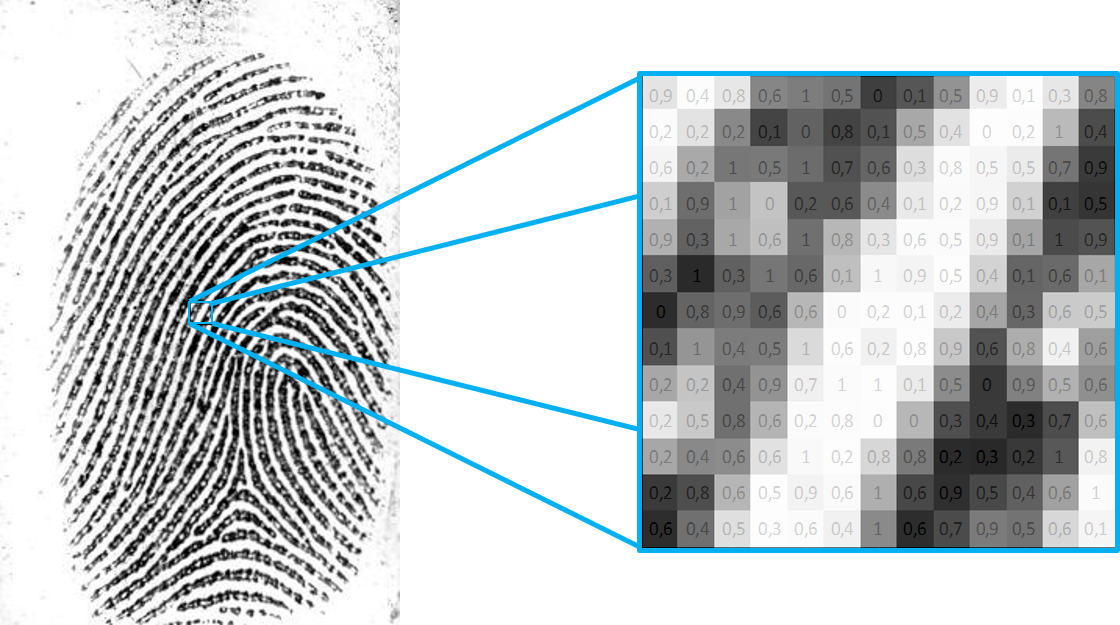
\includegraphics[scale=0.45]{figs/huella_pixeles_numeros.png}
        \caption{Huella Dactilar Digital}
    \end{figure}

\end{frame}

% ==== SLIDE 6 ====
\begin{frame}{Red Neuronal Convolucional}
    \begin{columns}[c] 
        \column{.42\textwidth}
        
            \begin{figure}[h]
                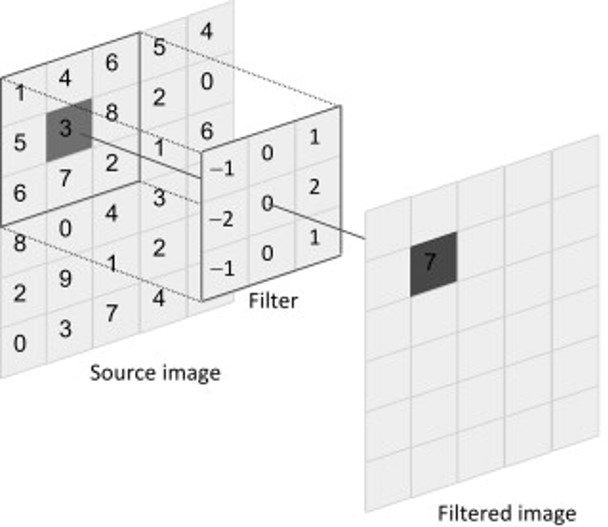
\includegraphics[scale=0.4]{figs/conv_2d.jpg}
                \caption{Proceso de Convolución}
            \end{figure}
            
        \column{.58\textwidth}
        
            \begin{itemize}
                \item Características de bajo y alto nivel.
                \vspace{4mm}
                
                \begin{figure}[h]
                    \begin{subfigure}{0.21\textwidth}
                        \centering
                        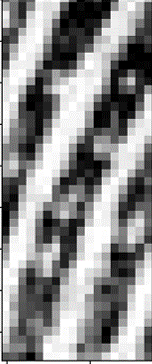
\includegraphics[scale=0.1]{figs/fll_0.png}  
                        \caption{Cresta Vertical}
                    \end{subfigure}
                    \begin{subfigure}{0.21\textwidth}
                        \centering
                        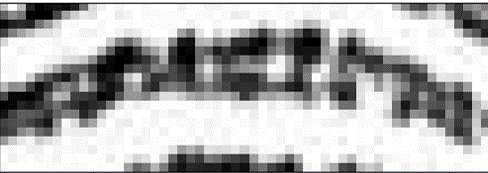
\includegraphics[scale=0.1]{figs/fll_1.png}  
                        \caption{Cresta Horizontal}
                    \end{subfigure}
                    \begin{subfigure}{0.21\textwidth}
                        \centering
                        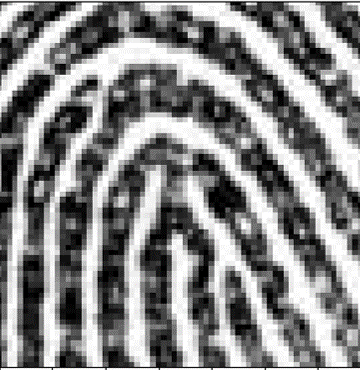
\includegraphics[scale=0.1]{figs/fhl_0.png}  
                        \caption{Núcleo}
                    \end{subfigure}
                    \begin{subfigure}{0.21\textwidth}
                        \centering
                        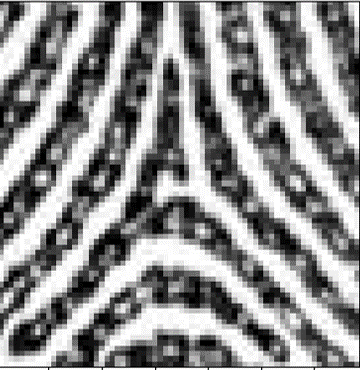
\includegraphics[scale=0.1]{figs/fhl_1.png}  
                        \caption{Delta}
                    \end{subfigure}
                \end{figure}
                
                \vspace{3mm}
                
                \item Parámetros:\\
                Modelo convolucional: 15 millones\\
                Perceptrón multicapa: 1000 millones
            \end{itemize}
            
    \end{columns}
\end{frame}

% ===


% ==== SLIDE 8 ====
\begin{frame}{Red Neuronal Convolucional}

   \begin{figure}[h]
        \begin{subfigure}{0.62\textwidth}
            \centering
            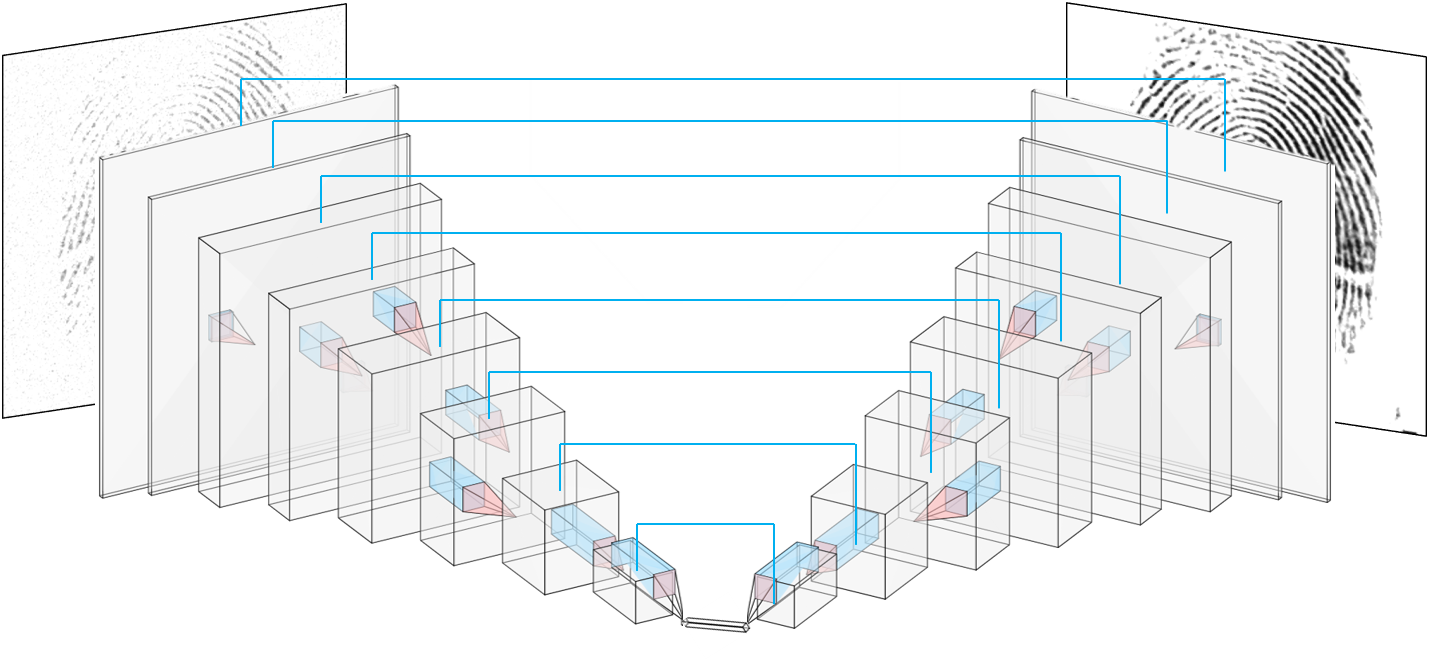
\includegraphics[scale=0.34]{figs/layers_nn_u.PNG}  
            \caption{Modelo de Reconstrucción Dactilar}
        \end{subfigure}
        \begin{subfigure}{0.36\textwidth}
            \centering
            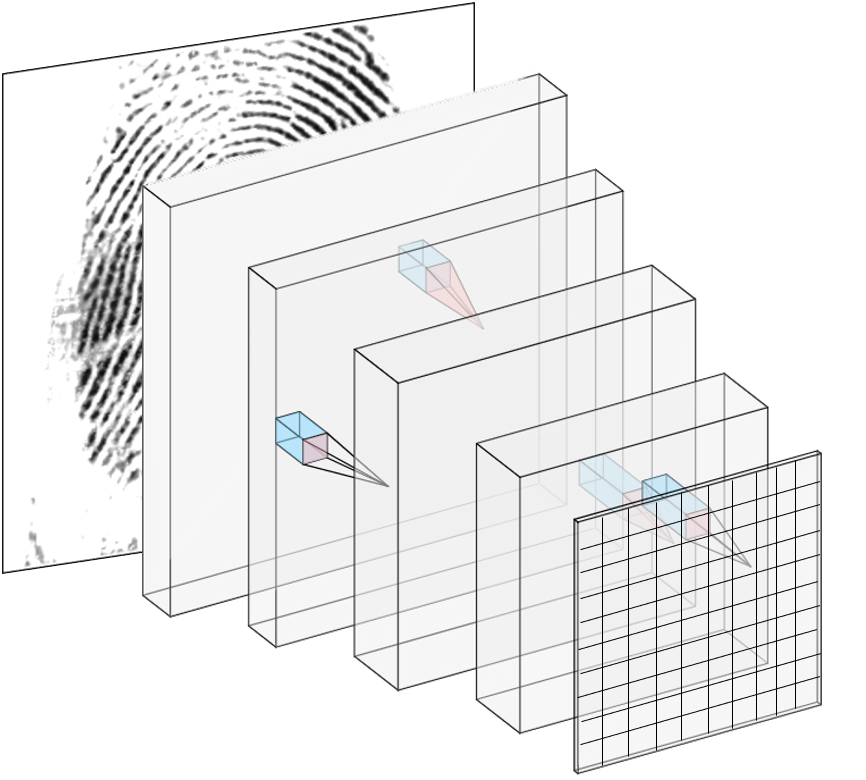
\includegraphics[scale=0.25]{figs/disc_cuad.png} 
            \caption{Discriminador Convolucional}
        \end{subfigure}
    \end{figure}

\end{frame}

% ==== SLIDE 10 ====
\begin{frame}{Entrenamiento del modelo}

    Olimpia facilitó 19.800 huellas digitales. Estas imágenes fueron deterioradas artificialmente para conformar el dataset utilizado en el proceso de entrenamiento.
    \vspace{5mm}

    \begin{figure}[h]
        \begin{subfigure}{0.48\textwidth}
            \centering
            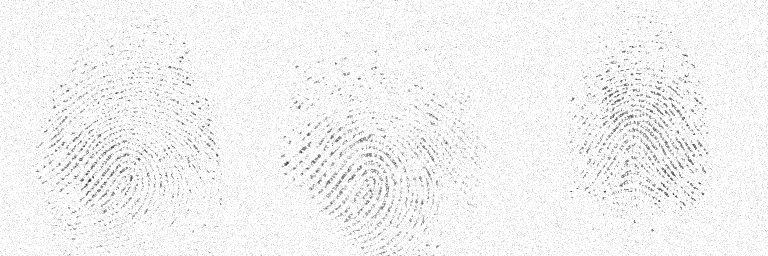
\includegraphics[scale=0.24]{figs/deterioration_2.png}  
            \caption{Deterioro por factor externo}
        \end{subfigure}
        \begin{subfigure}{0.48\textwidth}
            \centering
            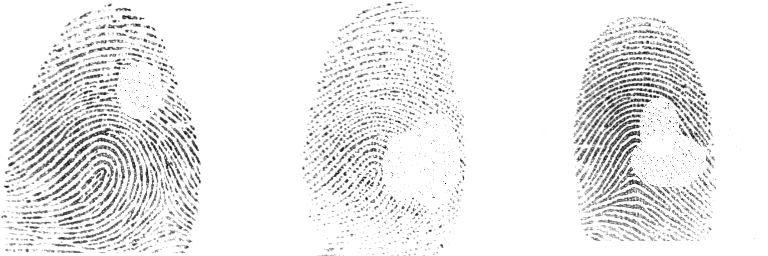
\includegraphics[scale=0.24]{figs/deterioration_1.png}  
            \caption{Deterioro de la piel}
        \end{subfigure}
    \end{figure}

\end{frame}

% ==== SLIDE 11 ====
\begin{frame}{Entrenamiento del modelo}

    \begin{figure}[h]
        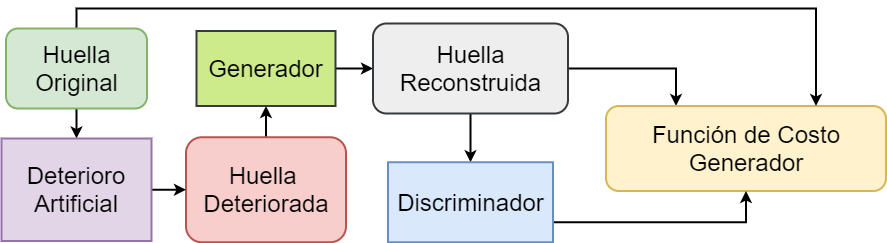
\includegraphics[scale=0.27]{figs/training_flow_gen.png}
        \caption{Cálculo de Costo del Generador}
    \end{figure}
    \vspace*{-5mm}
    \begin{figure}[h]
        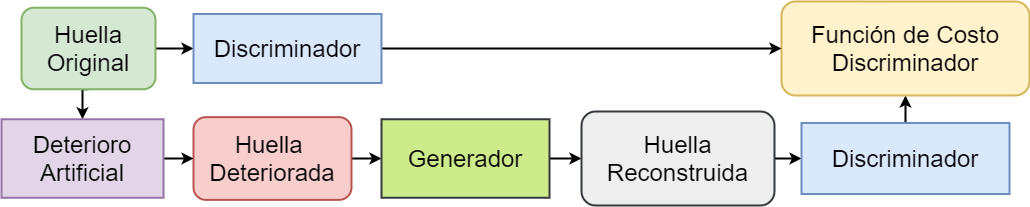
\includegraphics[scale=0.27]{figs/training_flow_disc.png}
        \caption{Cálculo de Costo del Discriminador}
    \end{figure}

\end{frame}

% ==== SLIDE 12 ====
\begin{frame}{Entrenamiento del modelo}

     Función de costo asociada al generador del modelo.
    \begin{equation}
        Gen_{loss} = \alpha||y-gen(x)||_{[1]} - log(disc(x,gen(x)))
    \end{equation}
    Función de costo asociada al discriminador del modelo.
    \begin{equation}
        Disc_{loss} = -log(1-disc(x,gen(x)))-log(disc(x,y))
    \end{equation}
    
    El parámetro \textit{y} corresponde a la huella original, \textit{x} a la huella deteriorada y $\alpha$ define el peso del componente reconstructivo en la expresión.

\end{frame}

% ===========
\begin{frame}{Entrenamiento del modelo}
    \begin{columns}[c] 
        \column{.7\textwidth}
        
            \begin{itemize}
                \item Para el desarrollo del modelo se utilizó Python y el framework de machine learning TensorFlow.
                \vspace{8mm}
                \item Se utilizó la unidad de procesamiento gráfico NVIDIA Tesla K40 disponible el cluster de cómputo de la Universidad de los Andes.
            \end{itemize}
            
        \column{.3\textwidth}
        
            \begin{figure}[h]
                
\includegraphics[scale=0.04]{figs/python}
            \end{figure}
            \vspace*{-4mm}
            \begin{figure}[h]
                
\includegraphics[scale=0.3]{figs/tensorflow.png}
            \end{figure}
            \vspace*{-7mm}
            \begin{figure}[h]
                
\includegraphics[scale=0.06]{figs/nvidia.png}
            \end{figure}
            
    \end{columns}
\end{frame}

% ==== SLIDE 14 ====
\begin{frame}{Resultados}

    \begin{figure}
        \begin{subfigure}{0.48\textwidth}
            \centering
            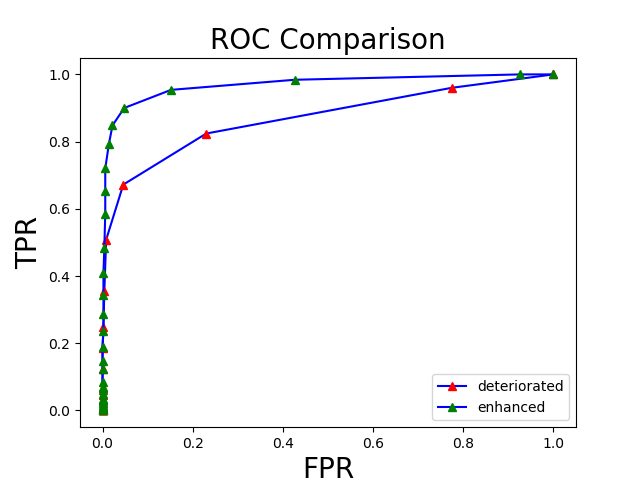
\includegraphics[scale=0.45]{figs/roc_comparison.png}
            \caption{Receiver Operating Characteristic}
        \end{subfigure}
        \begin{subfigure}{0.48\textwidth}
            \centering
            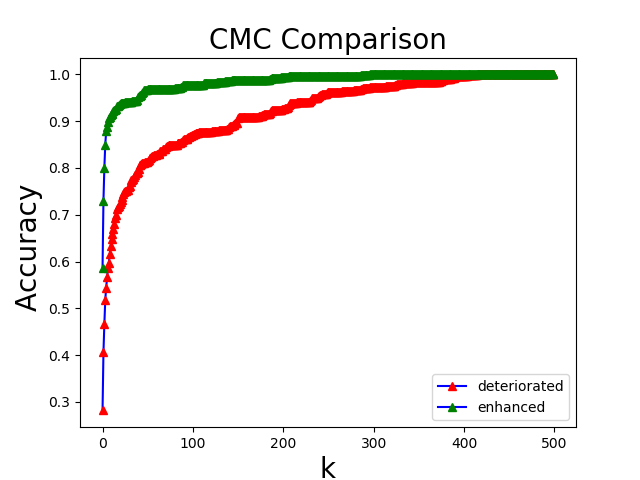
\includegraphics[scale=0.45]{figs/cmc_comparison.png}  
            \caption{Cummulative Match Curve}
        \end{subfigure}
    \end{figure}

\end{frame}

% ==== SLIDE 16 ====
\begin{frame}{Resultados}

    \begin{figure}[h]
        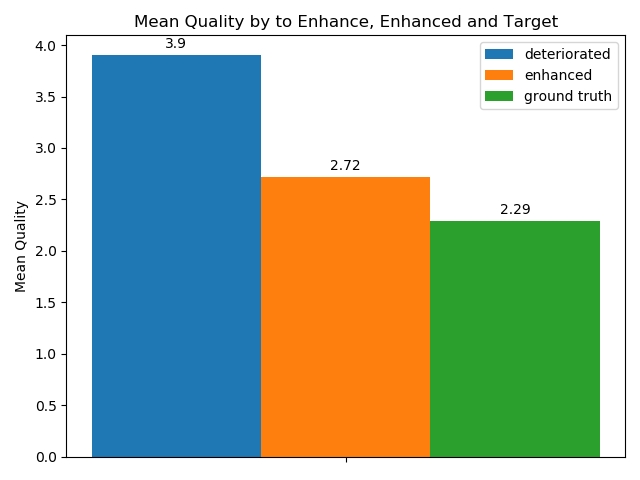
\includegraphics[scale=0.52]{figs/mean_qualities.png}
        \caption{Medida de Calidad de las Huellas}
    \end{figure}
    
\end{frame}

% ==== SLIDES REFERENCIAS ====
\nocite{*}
\begin{frame}[allowframebreaks]{Referencias}
\bibliographystyle{unsrt}
\bibliography{referencias.bib}
\end{frame}


% ==== ANEXOS ====
\begin{frame}{ANEXOS - Entrenamiento del modelo}

     Configuración del algoritmo de entrenamiento:
     \vspace{5mm}
     
     \begin{itemize}
        \item Batch size: 48
        \item Optimizador: ADAM.
        \item Beta 1: 0.5
        \item Beta 2: 0.999
        \item Tasa de aprendizaje: 0.00018
        \item $\alpha:$ 40
        \item Épocas: 96
    \end{itemize}
    
\end{frame}

\begin{frame}{ANEXOS -  Convolución y convolución Transpuesta}

    Lógica de la operación de convolución y convolución transpuesta en dos dimensiones aplicada a una imagen.

    \begin{figure}[h]
        \begin{subfigure}{0.45\textwidth}
            \centering
            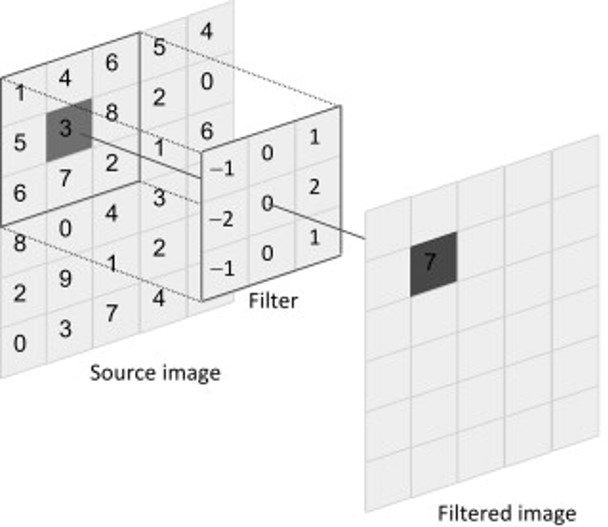
\includegraphics[scale=0.325]{figs/conv_2d.jpg}  
            \caption{Convolución}
        \end{subfigure}
        \begin{subfigure}{0.45\textwidth}
            \centering
            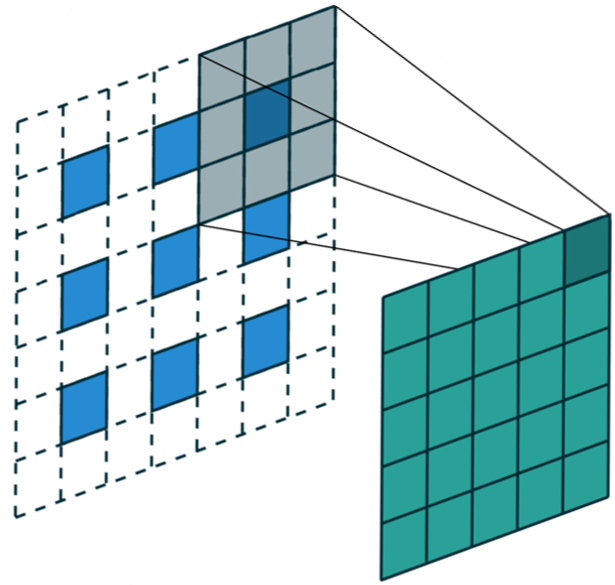
\includegraphics[scale=0.30]{figs/trans_conv.PNG}  
            \caption{Convolución Transpuesta}
        \end{subfigure}
    \end{figure}

\end{frame}

\end{document}